\documentclass{jib}
\newlength{\platz}
\setlength{\platz}{15pt}
\RequirePackage{listings}

%\usepackage{changepage} %test, TODO remove

\lstset{%
  basicstyle=\ttfamily,
  fontadjust,
  flexiblecolumns=true,
  frame=L,
  xleftmargin=15pt,
  framesep=5pt,
  emphstyle=\rmfamily\itshape}
  

\usepackage{pdfpages}

%%%%%%%%%%%%%%%%%%%%%%%%%%%%%%%%%%%%%%%%%%%%%%%%%%%%%%%%%%
% JIB Header/Footer
%%%%%%%%%%%%%%%%%%%%%%%%%%%%%%%%%%%%%%%%%%%%%%%%%%%%%%%%%%
\jibvolume{XX} % insert volume
\jibissue{X}   % insert issue
\jibpages{XXX} % insert article ID
\jibyear{XXXX} % insert year
\makeHeaderFooter{} % leave as is
%%%%%%%%%%%%%%%%%%%%%%%%%%%%%%%%%%%%%%%%%%%%%%%%%%%%%%%%%%

\begin{document}

%%%%%%%%%%%%%%%%%%%%%%%%%%%%%%%%%%%%%%%%%%%%%%%%%%%%%%%%%%
%
% Title Page
%
%%%%%%%%%%%%%%%%%%%%%%%%%%%%%%%%%%%%%%%%%%%%%%%%%%%%%%%%%%

\begin{jibtitlepage}

\jibtitle{Synthetic Biology Open Language Visual (SBOL Visual) \\ Version 3.0}


%We did not provide author(s) nor author footnote(s), please complete as applicable.
% Please make sure to use unique footnote characters for each author
\jibauthor{
Hasan Baig\iref{uconn},
Pedro Fontanarossa\iref{utah},
James McLaughlin\iref{embl},
James Scott-Brown\iref{oxford},
Prashant Vaidyanathan\iref{msr},
Thomas Gorochowski\iref{bristol}, 
Goksel Misirli\iref{keele},
Jacob Beal\iref{bbn},
Chris Myers\iref{ucb}\jibauthorfootnote{*}{Correspondence should be addressed to:
           \email{editors@sbolstandard.org}}}

\addjibinstitution{uconn}{University of Connecticut, USA}
\addjibinstitution{utah}{University of Utah, USA}
\addjibinstitution{embl}{EMBL-EBI, UK}
\addjibinstitution{oxford}{University of Oxford, UK}
\addjibinstitution{msr}{Microsoft Research, UK}
\addjibinstitution{bristol}{University of Bristol, UK}
\addjibinstitution{keele}{Keele University, UK}
\addjibinstitution{bbn}{Raytheon BBN Technologies, USA}
\addjibinstitution{ucb}{University of Colorado Boulder, USA}

\end{jibtitlepage}


\begin{abstract}

People who engineer biological organisms often find it useful to draw diagrams in order to communicate both the structure of the nucleic acid sequences that they are engineering and the functional relationships between sequence features and other molecular species. 
Some typical practices and conventions have begun to emerge for such diagrams. 
SBOL Visual aims to organize and systematize such conventions in order to produce a coherent language for expressing the structure and function of genetic designs. 

This document details version 3.0 of SBOL Visual, a new major revision of the standard.
The major difference between SBOL Visual 3 and SBOL Visual 2 is that diagrams and glyphs are defined with respect to the SBOL 3 data model rather than the SBOL 2 data model.
A byproduct of this change is that the use of dashed undirected lines for subsystem mappings has been removed, pending future determination on how to represent general SBOL 3 constraints; in the interim, this annotation can still be used as an annotation.
Finally, deprecated material has been removed from collection of glyphs: the deprecated ``insulator'' glyph and ``macromolecule'' alternative glyphs have been removed, as have the deprecated BioPAX alternatives to SBO terms.
\end{abstract}

This document does not contain technology or technical data controlled under either the U.S. International Traffic in Arms Regulations or the U.S. Export Administration Regulations.

\textbf{Keywords:} SBOL Visual; Standards; Diagrams

% Include your PDF document
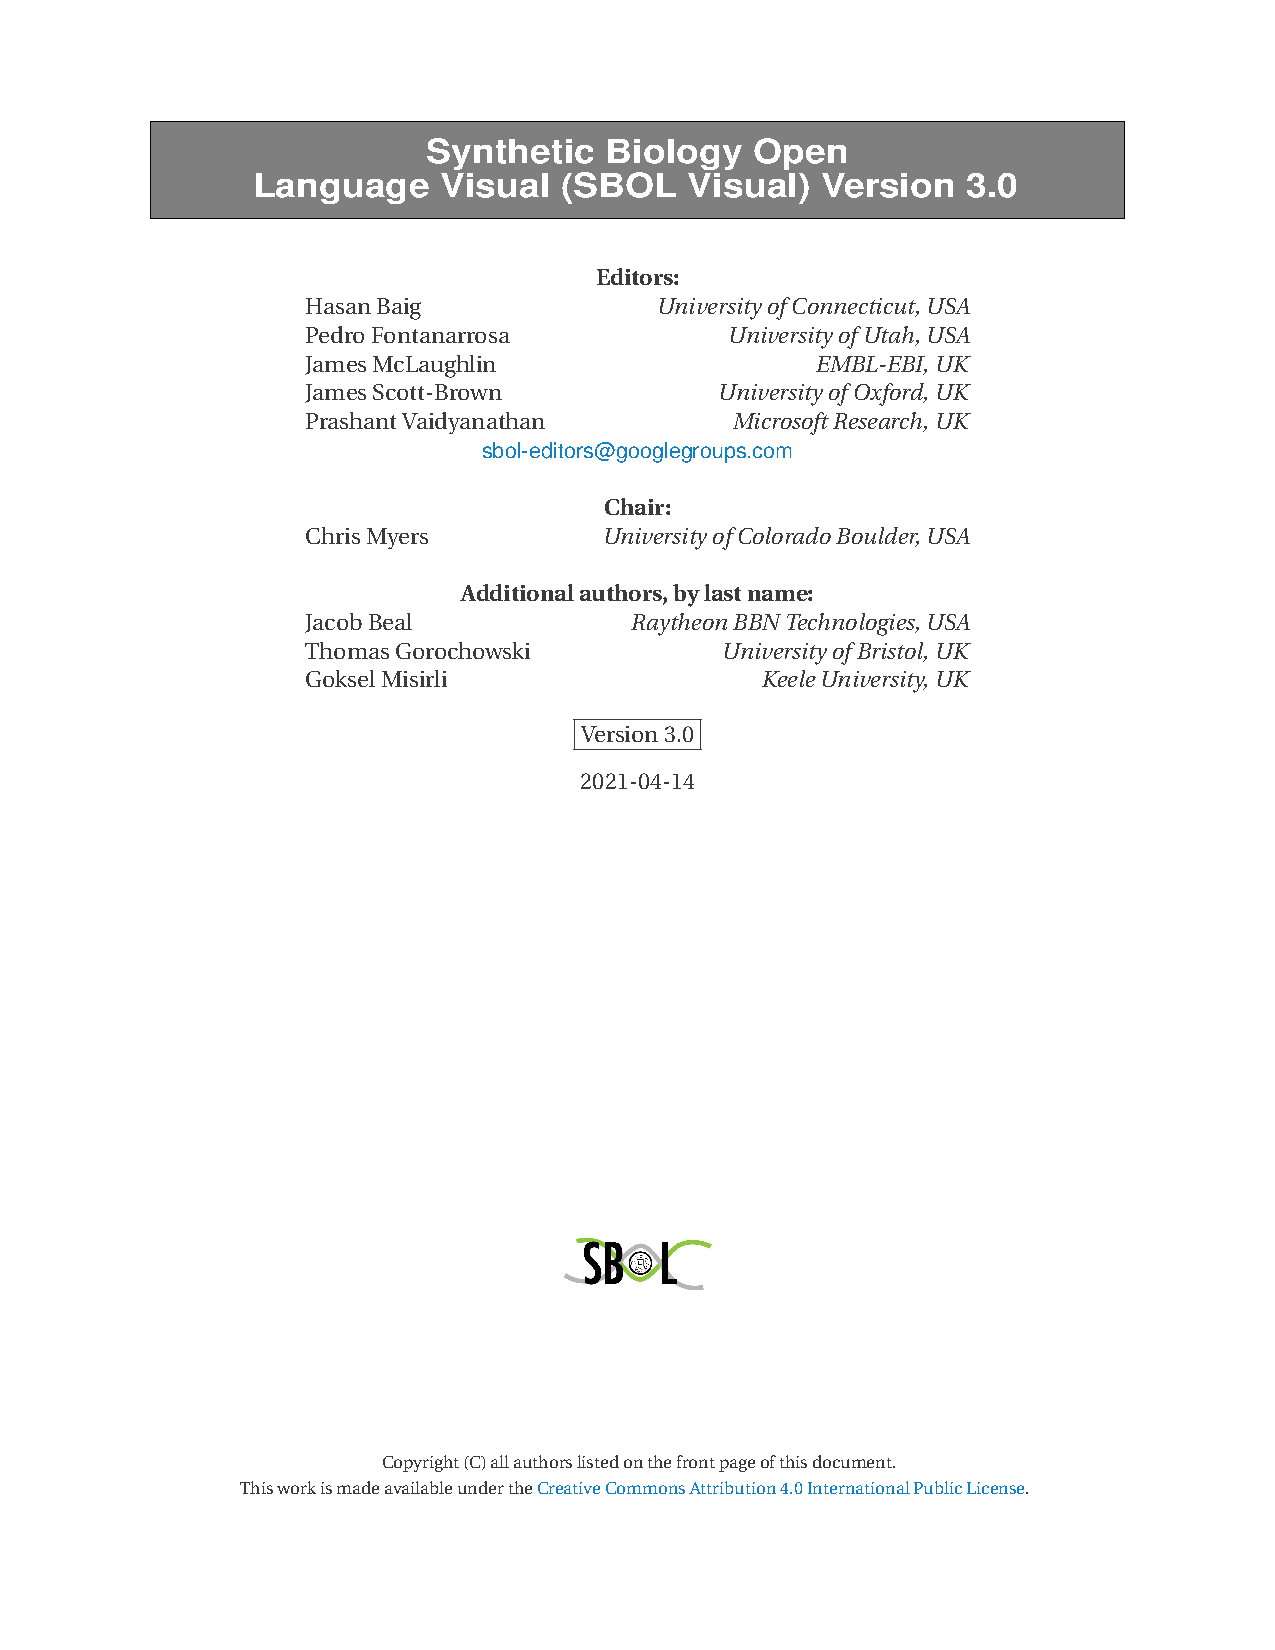
\includepdf[pages=-, offset=80 -80]{SBOL_Visual_3_0.pdf}

\end{document}
